%%%%%%%%%%%%%%%%%%%%%%%%%%%%% TCC %%%%%%%%%%%%%%%%%%%%%%%%%%%%%%%%
%
% Template para TCC da Universidade Federal da Paraíba
%
% Autores: Elaine Soares elaineanita1@gmail.com
%          Rafael Brayner rafabrayner92@gmail.com
%          Roberto Júnior contato@robertojunior.net
%
% ShareLaTeX porting: Gustavo Sobral ghsobral@gmail.com
% 
% Revisão: Eudisley Anjos eudisley@ci.ufpb.br
%
% Sinta-se livre para melhorar e contribuir com esse projeto. 
%
%%%%%%%%%%%%%%%%%%%%%%%%%%%%%%%%%%%%%%%%%%%%%%%%%%%%%%%%%%%%%%%%%%%

\documentclass{tcc}
\bibliographystyle{plain}
\usepackage{etoolbox}
\usepackage{ragged2e} 
\usepackage{siunitx}
\justifying
\patchcmd{\thebibliography}{\section*{\refname}}{}{}{}
\usepackage{titlesec}
\setcounter{tocdepth}{4}
\setcounter{secnumdepth}{7}
 \usepackage{mathptmx} 
\usepackage[linkcolor = black, colorlinks = true,citecolor=black,urlcolor=blue,bookmarks=false,hypertexnames=false]{hyperref} 
\linespread{1.25}

\begin{document}
\pagestyle{empty} %retira numeração da página
%Dados do TCC%

\author{\\  Pedro Paulo Costa Castro Alves \hspace{1cm}  11721ECP017 }
\title{Universidade Federal de Uberlândia}
\newcommand{\subtitulo}{Faculdade de Engenharia Elétrica - FEELT}
\newcommand{\nomedocurso}{Engenharia de Computação}
\newcommand{\titulobar}{}
\newcommand{\orientador}{Nome do Orientador}
\newcommand{\profa}{Nome do Professor A}
\newcommand{\profb}{Nome do Professor B}
\newcommand{\profc}{Nome do Professor C}
\newcommand{\insta}{Instituicao do Professor A}
\newcommand{\instb}{Instituicao do Professor B}
\newcommand{\instc}{Instituicao do Professor C}
\newcommand{\coordenador}{Nome do Coordenador}
\newcommand{\departamento}{Nome do Departamento}
\renewcommand{\contentsname}{Índice}

\begin{center}
\Huge{\bf \thetitle}\\~\\
\begin{figure}[H]
\centering

\includegraphics{imagens/UFU.png}
\end{figure}
\huge{\bf \subtitulo}\\~\\
\Large{\bf Trabalho VI - Adaline}\\~\\

\end{center}

\vspace{2em}

\begin{center}
Prof.: Dr. Keiji Yamanaka

\end{center}

\vspace{2em}
\begin{table}[htb]
\centering
\begin{tabular}{ccc}
Aluno                           &  & Matrícula   \\
                                &  &             \\
Pedro Paulo Costa Castro Alves  &  & 11721ECP017 \\
\end{tabular}
\end{table}


\vspace{5cm}


\begin{center}
Uberlândia, 15 de Junho de 2021
\end{center}
\clearpage
\setcounter{page}{1}


%Índice%

\pagestyle{plain} %mostra numeração da página%

\newpage
\section{Introdução}
Usaremos o algoritmo de RNA's "Adaline" para calcular a regressão linear de um conjunto de dados.

\section{Dados}
Este é o conjunto de dados os quais trabalharemos, determinaremos coeficientes de correlação, determinação, regressão e intercepto.
	\begin{table}[H]
		\center
	\begin{tabular}{|c|c|}
		\hline
		x    & y     \\ \hline
		0.00 & 2.26  \\ \hline
		0.50 & 3.80  \\ \hline
		1.00 & 4.43  \\ \hline
		1.50 & 5.91  \\ \hline
		2.00 & 6.18  \\ \hline
		2.50 & 7.26  \\ \hline
		3.00 & 8.15  \\ \hline
		3.50 & 9.14  \\ \hline
		4.00 & 10.87 \\ \hline
		4.50 & 11.53 \\ \hline
		5.00 & 12.55 \\ \hline
	\end{tabular}
\end{table}

Após o uso do software BioEstat, que usa as fórmulas estatísticas para calcular seus resultados, chegou-se aos seguintes:

\begin{figure}[H]
	\center
	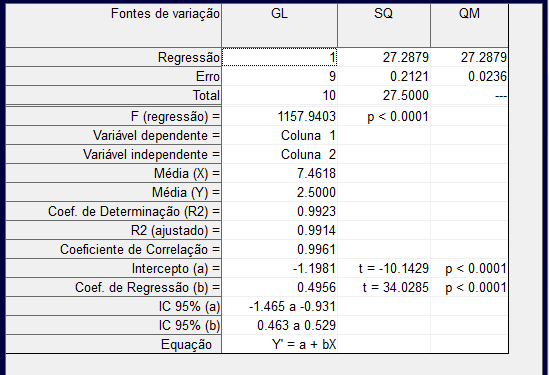
\includegraphics[scale=0.7]{imagens/reglin.png}
	\caption{Dados calculados pelo BioEstat.}
\end{figure}

\begin{figure}[H]
	\center
	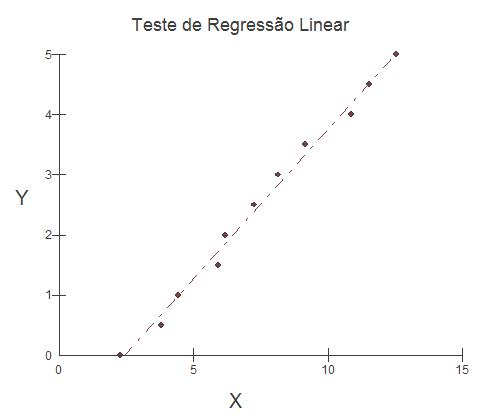
\includegraphics[scale=1]{imagens/graflin.png}
	\caption{Gráfico gerado pelo BioEstat.}
\end{figure}

Coeficiente de Regressão (Coeficiente Angular da reta): 0.4956\\
Coeficiente de Correlação: 0.9961\\
Intercepto (Coeficiente Linear): -1.1981\\
Coeficiente de Determinação: 0.9923\\


\subsection{O Programa}

O algoritmo da rede neural do Adeline será implantada através de um simples programa de computador escrito na linguagem C.


\subsection{Testando o Programa}

\begin{figure}[h]
	\center
	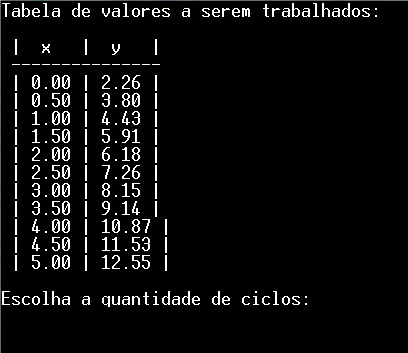
\includegraphics[scale = 1]{imagens/interf.png}
	\caption{Interface do Programa}
\end{figure}

O programa nos permite escolher a quantidade de ciclos e se os tratamento dos dados será apresentados em tempo real de execução ou se queremos apenas os resultados finais.

\begin{figure}[H]
	\center
	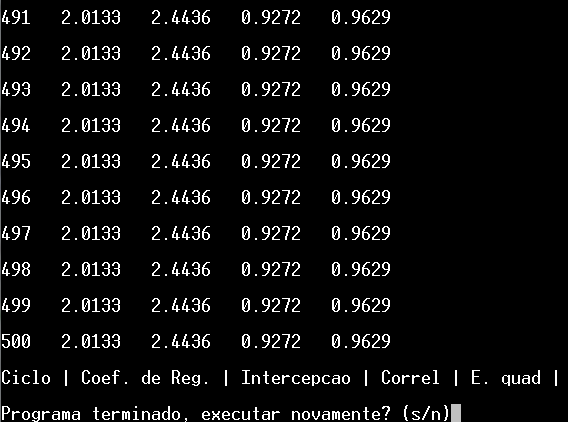
\includegraphics[scale =0.9]{imagens/real.png}
	\caption{Dados em tempo real para 500 ciclos.}
\end{figure}

\begin{figure}[H]
	\center
	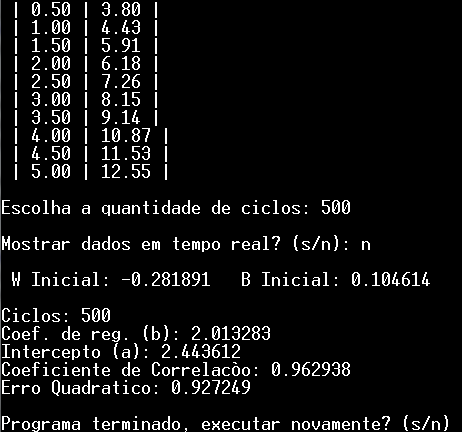
\includegraphics[scale =1]{imagens/estat.png}
	\caption{Apenas a saída final, para 500 ciclos.}
\end{figure}

Utilizando um ciclo bem alto (ordem de $10^6$), os valores permaneceram inalterados, quando comparados com 500 ciclos, o que garante que estes são os valores finais:

Coeficiente de Regressão (Coeficiente Angular da reta): 2.0133\\
Coeficiente de Correlação: 0.9272\\
Intercepto (Coeficiente Linear): 2.44636\\
Coeficiente de Determinação: 0.9629

Comparando com os dados obtidos pelo BioEstat observamos coeficientes de correlação e 
de determinação bem próximos, porém o restante divergiu por muito.


\end{document}